\begin{priprava}{8., 9}{}{Grafično prikazovanje podatkov}{Osnove statistike}{frontalna, delo v dvojicah/individualno}{drsnice, projekcija, računalniki}

    \section{Grafično prikazovanje podatkov}
                

    \subsection*{Strukturni krog}
    
        \textbf{Strukturni krog} ali \textbf{krožni diagram} uporabljamo, kadar so podatki razvrščeni v malo frekvenčnih razredov 
        ali ne dosežejo veliko različnih diskretnih vrednosti.
    
        \begin{figure}[H]
            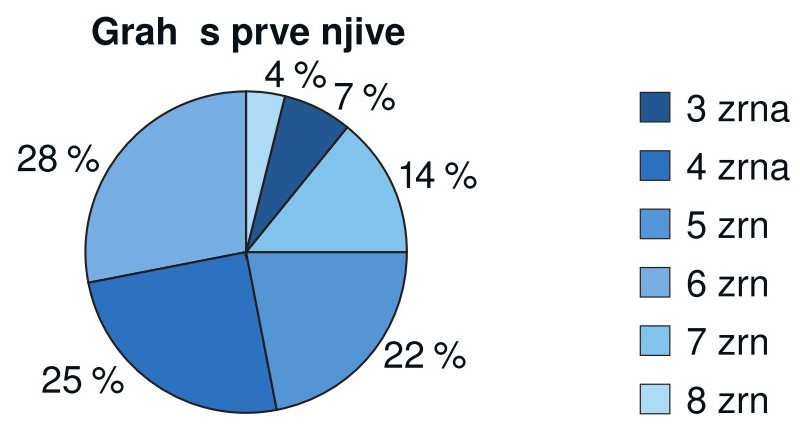
\includegraphics[scale=0.3]{../../Slike_in_skice/10921.jpg}
            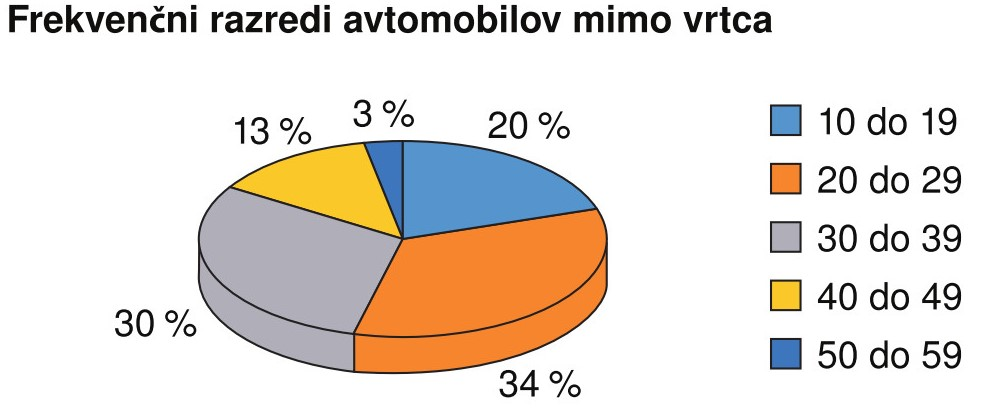
\includegraphics[scale=0.3]{../../Slike_in_skice/1092.jpg}
        \end{figure}

    
        Celoto predstavlja $360^\circ$, za ostale deleže središčne kote izračunamo s sklepnim računom.
    
        ~

    \subsection*{Stolpčni diagram}

        \textbf{Stolpčni diagram} uporabljamo, ko so podatki razvrščeni v veliko frekvenčnih razredov
        ali lahko dosežejo veliko diskretnih vrednosti.
        
        ~
            
        Stolpčni diagrami so lahko \textbf{pokončni} ali \textbf{ležeči}. 
        Če želimo prikazati več podatkov naenkrat, uporabimo \textbf{sestavljeni} ali \textbf{strukturni} stolpčni diagram.
    
        
        \begin{figure}[H]
            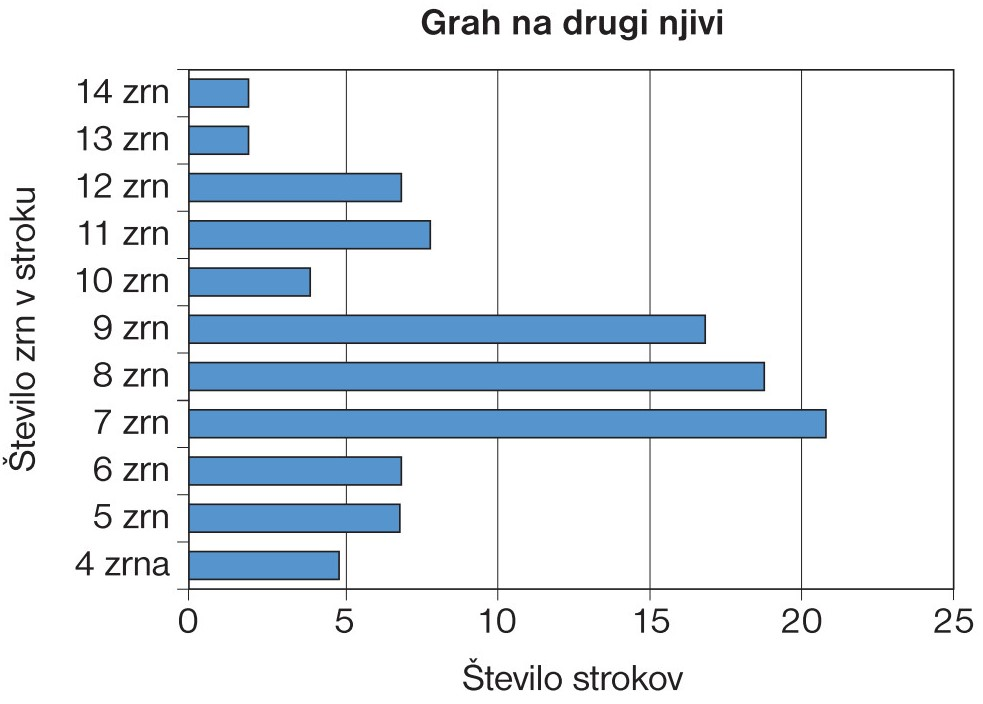
\includegraphics[scale=0.3]{../../Slike_in_skice/1093.jpg}
            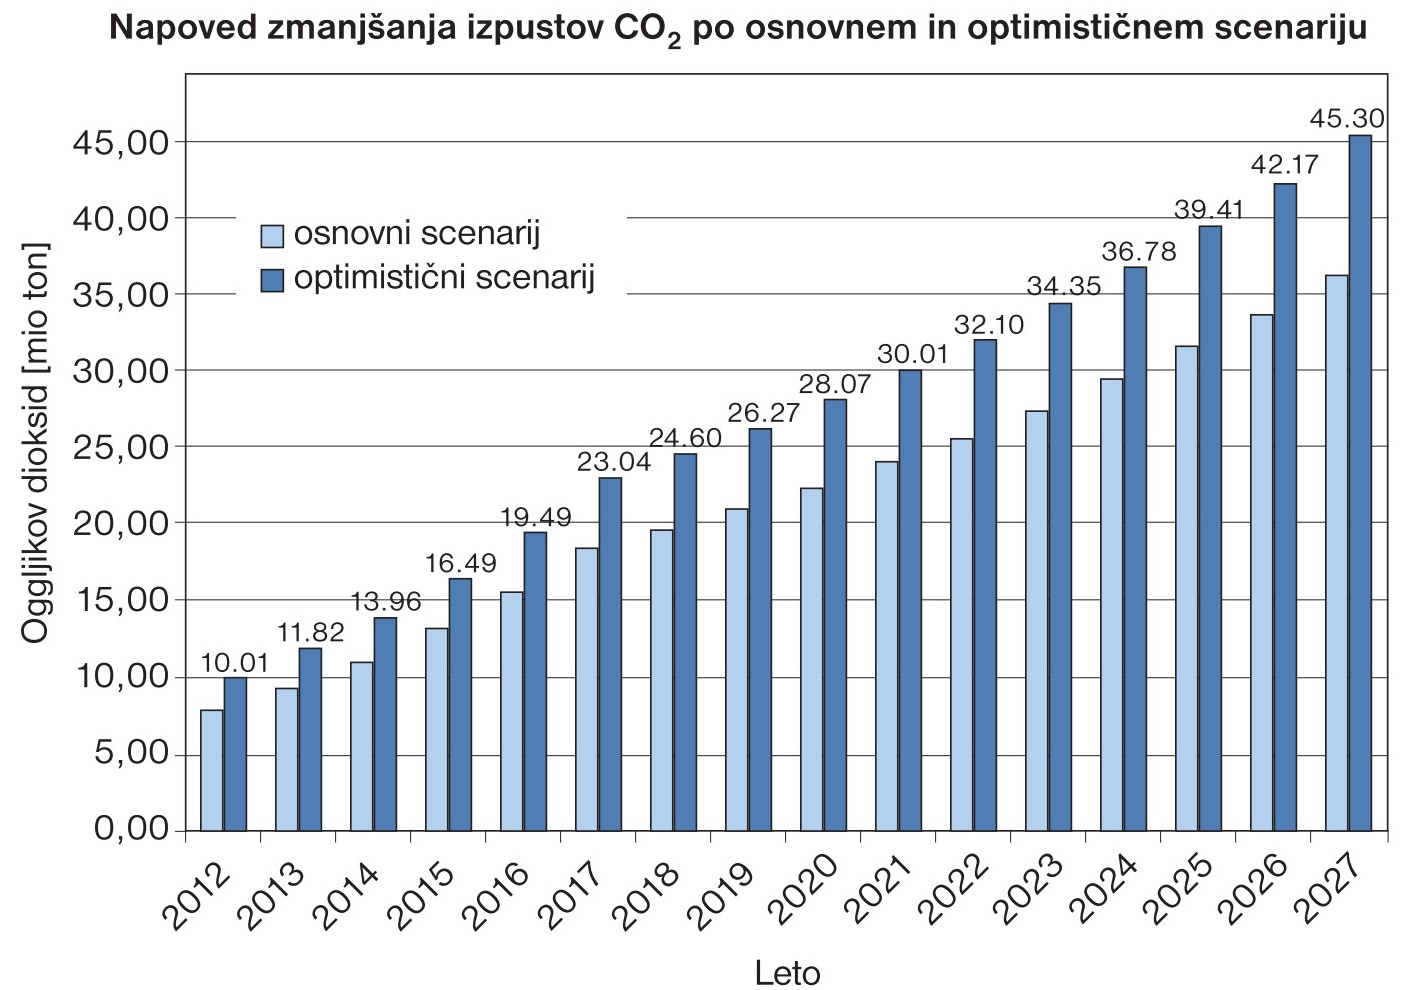
\includegraphics[scale=0.22]{../../Slike_in_skice/1095.jpg}
            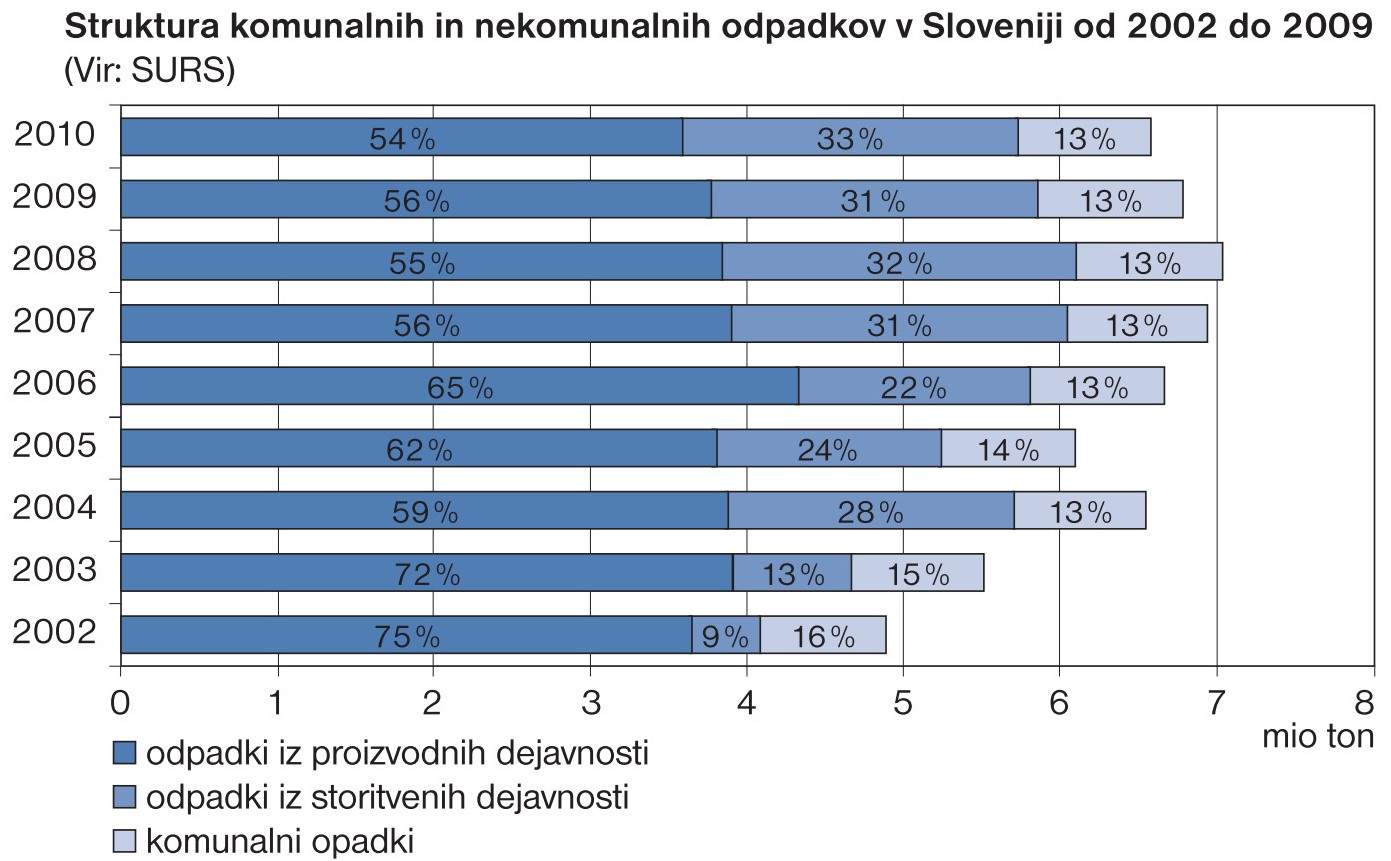
\includegraphics[scale=0.22]{../../Slike_in_skice/1097.jpg} 
            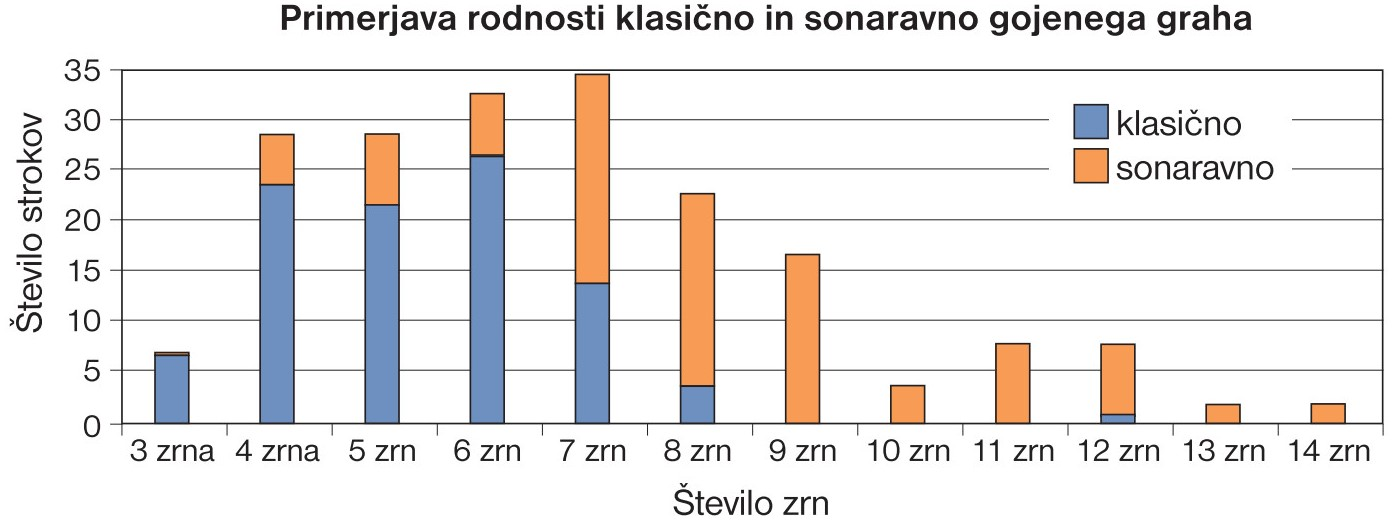
\includegraphics[scale=0.21]{../../Slike_in_skice/1096.jpg}
            
        \end{figure}
    




\newpage

\subsection*{Histogram}

    \textbf{Histogram} uporabljamo za prikaz grupiranih podatkov. 

        \begin{figure}[H]
            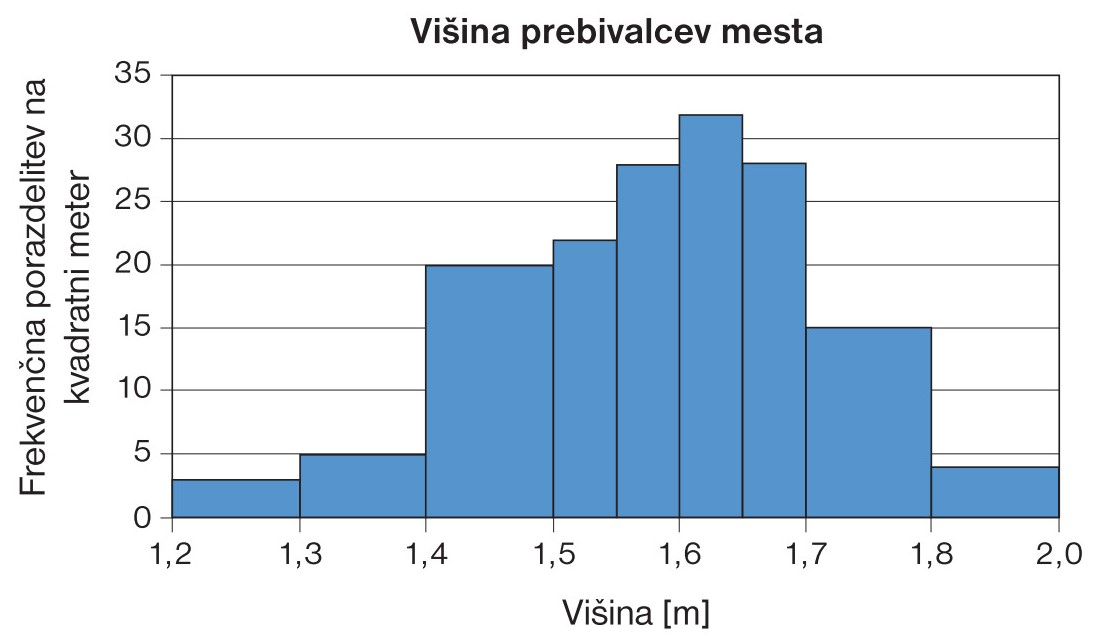
\includegraphics[scale=0.33]{../../Slike_in_skice/1098.jpg}
        \end{figure}


    Širine frekvenčnih razredov niso nujno enake.
    Meje razredov narišemo na vodoravni osi, frekvence posameznih razredov pa na navpični osi.



            




~

\subsection*{Linijski diagram}

    \textbf{Linijski diagram/poligon} uporabljamo, ko želimo prikazati postopno spreminjanje vrednosti nekega podatka skozi daljše časovno obdobje.
    Frekvenčne porazdelitve ponazorimo s \textbf{frekvenčnim poligonom}, podatki so lahko zvezni ali grupirani.
        
            \begin{figure}[H]
                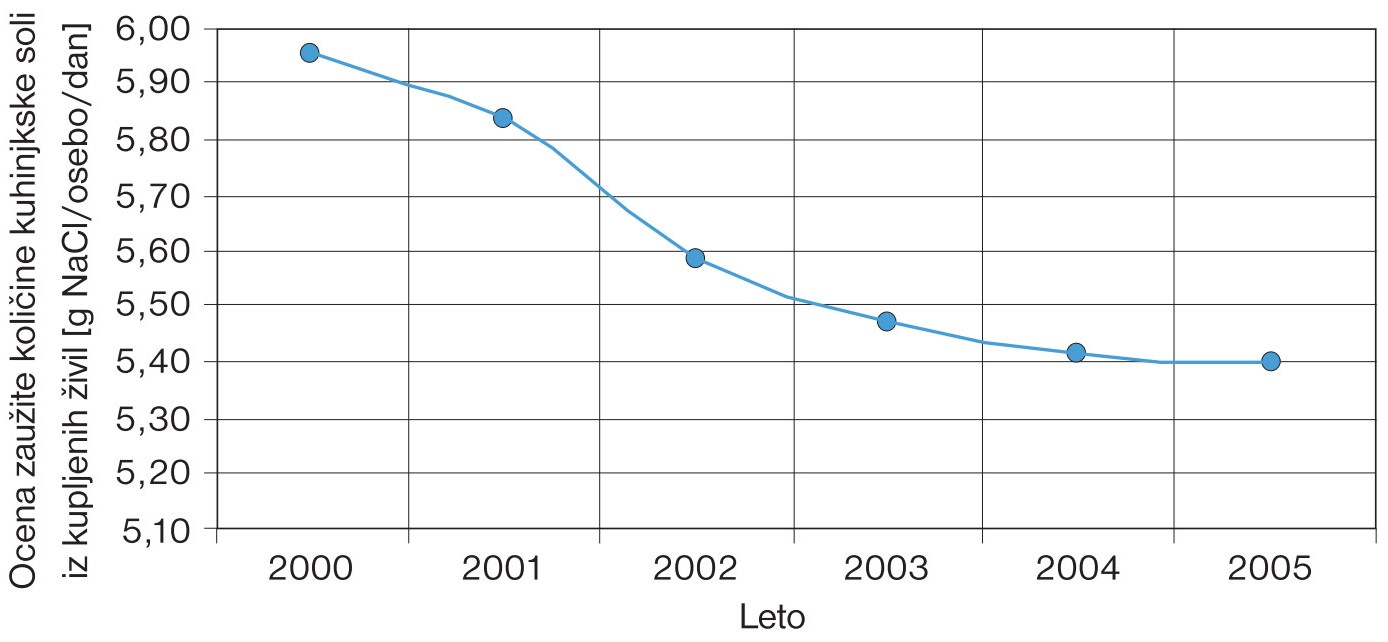
\includegraphics[scale=0.23]{../../Slike_in_skice/1166.jpg}
                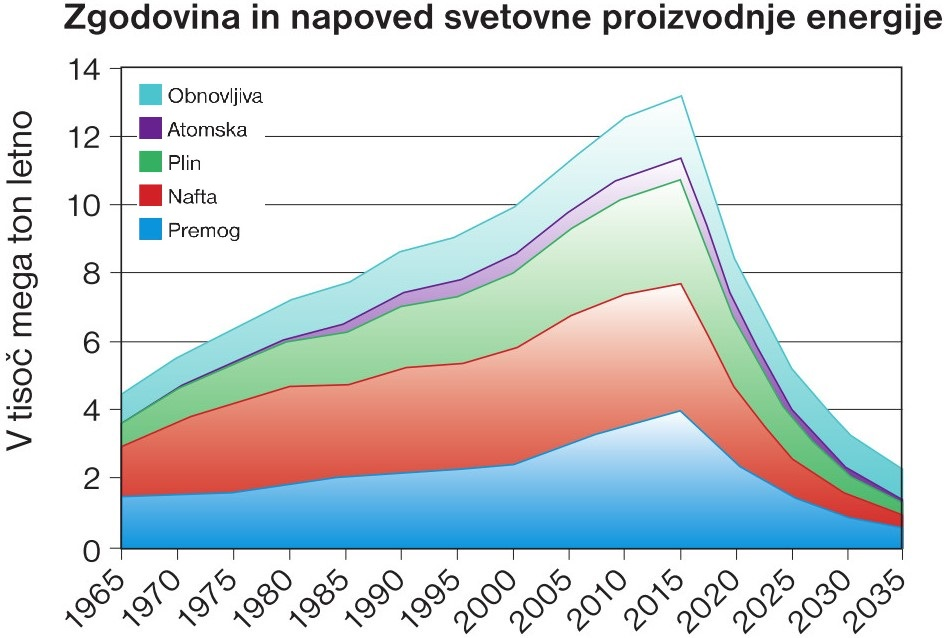
\includegraphics[scale=0.3]{../../Slike_in_skice/1099.jpg}
            \end{figure}
            

~\\~\\~


%%%% naloge




    \begin{naloga}
 
        Na matematičnem testu je bilo mogoče doseči $50$ točk. Dosežki so bili: 
        $35, 22, 41, 47$, $36, 30, 27, 19, 31, 43, 48, 44, 23, 26, 36, 10, 33, 14, 9$. \\
        Razdelite jih v pet enako velikih razredov ter predstavite s histogramom.
        
    \end{naloga}


    \begin{naloga}
     
     Otroci v vrtcu so metali žogo na koš in si zapisovali dosežke. Podatki so prikazani v preglednici. 

         \begin{table}[H]
             \centering
             \begin{tabular}{||c|c|c|c|c|c|c|c|c|c||} 
             \hhline{|t:==========:t|}
             \rowcolor[rgb]{0.843,0.718,0.718} 
             Otrok  & Jaka & Jure & Miha & Polona & Valerija & Tina & Mojca & Cene & Darja   \\ 
             \hhline{|:==========:|}
             Št.~košev & $5$ & $7$ & $10$ & $8$ & $5$ & $6$ & $9$ & $9$& $4$  \\ 
             \hhline{|b:==========:b|}
             \end{tabular}
         \end{table}

         Izračunajte, koliko košev je otrok zadel v povprečju. Podatke uredite po vrsti in določite $Mo$, $Me$ ter narišite škatlo z brki.

    \end{naloga}





\begin{naloga}
 
    Bojana beleži, koliko časa potrebuje za pot do šole. Podatke je zapisala v preglednico. 

     \begin{table}[H]
         \centering
         \begin{tabular}{||c|c|c|c|c|c|c|c|c|c|c||} 
         \hhline{|t:===========:t|}
         \rowcolor[rgb]{0.843,0.718,0.718} 
         Dan  & 1. & 2. & 3. & 4. & 5. & 6. & 7. & 8. & 9. & 10.   \\ 
         \hhline{|:===========:|}
         Čas [min] & $9$ & $11$ & $10$ & $8$ & $11$ & $10$ & $9$ & $12$& $9$ & $11$ \\ 
         \hhline{|b:===========:b|}
         \end{tabular}
     \end{table}

     S stolpčnim diagramom predstavite, kako pogosto v šolo potuje $8$ minut, $9$ minut ... 

\end{naloga}

\begin{naloga}
 
    V domu ostarelih občanov je $500$ oskrbovancev. Od $50$ do $60$ let jih je $15~\%$, med $60$ in $70$ leti je $160$ oskrbovancev,
    med $70$ in $80$ leti pa $200$ starostnikov. Drugi so stari med $80$ in $90$ let.
    \begin{itemize}
        \item Iz grupiranih podatkov izračunajte povprečno starost oskrbovancev tega doma.
        \item Grafično ponazorite starost oskrbovancev.
    \end{itemize}
    
\end{naloga}




\end{priprava}